\documentclass[12pt]{article}
\usepackage[margin=1in]{geometry}
\usepackage{ifpdf}
\usepackage{mla}
\usepackage{booktabs}
% \usepackage{mathtools}

\usepackage{caption}
\captionsetup{labelsep=period}
\renewcommand{\figurename}{Fig.}

\usepackage[normalem]{ulem}

% Widow and orphan penalty.
\widowpenalty=10000
\clubpenalty=10000

\begin{document}
\begin{mla}{Colby}{Goettel}{Reed}{English 312}{18 March 2014}{Telecommunication Monopolies and Broadband Infrastructure}
% most of the order needs to be drastically changed

% Intro, contract: WATCO the merger on BI?
% REWORD
This year, Comcast announced that it will be buying Time Warner Cable for a staggering \$45B. This merger between the two largest telecommunications companies in the United States will create a monopoly [similar to Bell Labs before its dissolution.] [This monopoly, the merger of two corporations notorious for their poor customer service and lack of commitment to providing quality infrastructure, will only further delay the building of proper broadband infrastructure in the United States, thus further pulling us into the Stone Age. Some argue these points, but what will be the actual effect of this merger on the Unites States' broadband infrastructure?]

% A: merger
In early February, Comcast announced a bid to buy Time Warner Cable in an all-stock deal of more than \$45B. Comcast and Time Warner Cable, both cable television and Internet service providers, are the two largest cable companies in the United States. Their merger would create a monopoly on telecommunications in the United States.

This merger still needs regulatory approval, but the cards seem to be stacked in favor of it. Congress does not see this as an antitrust issue. Politico recently reported that 15/18 members of the Senate Judiciary Committee and 32/39 members of the House Judiciary Committee have received a donation from Comcast. This is legal bribery. This will ensure that Comcast will have its way throughout the hearings (Romm). Incredulously, Comcast has spoken up about this bribery saying that it is simply them being involved in the political process (Sottek). They have brazenly committed bribery and have brazenly dismissed their actions as natural, regular, part of the political process.

% this is essential:
% talk about history with Ma Bell
% how monopolies do not do what the customers want


% I think these two areas will bleed a lot into each other (so keep them close and don't try to hard to compartmentalize)
% C: tight regulations that don't allow for advancement
% A->C: merger's effects on regulations
% anti-trust
% bribing congress
% venezia: this is where backwoods America should be right now

% comcast and utopia. From Ekstrom:
% Obviously the legislature would argue that ``cities shouldn't compete with private industry'' protected monopolies don't like competition.
% You would have to follow the money in the 2000-2005 period to see it. No reporter cared enough to document it. Most of the reporting has been iProvo and Utopia are dumb ideas that got the cities into debt, not why is Utah valley booming right now?
% Short answer, I don't know of any analysis of the political implications of the legal environment.
The past decade of broadband infrastructure in Utah illustrates a great example of what happens to competition when monopolies exist. In the mid-2000s, seventeen Utah cities joined forces to provide quality fiber infrastructure to their residents. Their consortium is called the Utah Telecommunication Open Infrastructure Agency, or Utopia. The cities laid fiber optic cable and currently provide service to over 11,000 subscribers. Comcast didn't like the competition and paid off the Utah legislature to make it legal for cities to lay infrastructure, but illegal for them to advertise their service.

Provo announced last year that Google Fiber would be buying their existing infrastructure. This deal cost a grand total of \$1. Provo tried to sell for almost \$300M, but Google said that they would pay \$1, nothing more, but would improve the existing infrastructure with almost \$500M of work. This deal ended the city and its citizens from having to pay further taxes to pay off the infrastructure and will greatly improve the infrastructure in Provo.

However, unknown to most, Utopia actually provides better and cheaper service than Google Fiber. But they're not allowed to advertise it because Comcast paid off the legislature to make this illegal.

Fortunately, because Google Fiber is coming to Provo and improving infrastructure, they have forced Comcast to improve their service or be left in the dust. Comcast has since been going to existing customers and giving them free cable television and 50Mbps Internet. The disgusting thing is that they have had the infrastructure in place for years to offer this kind of service, but didn't because there was no competition. Why the hell should any of their customers remain faithful to a company that has swindled them for years?

% B: infrastructure
% make sure it's explicit that this will limit both the current infrastructure (for money) as well as the future infrastructure
% need to bury cables whenever you're underground (10x the cost)
% reference the table and figure

% glass single-mode fiber - ``But I have also done the calculations myself, using Shannon's Law, and (as I showed in class) a single strand of single-mode fiber (not multi-mode) has enough bandwidth to allow for 10 Gbps for every person on the planet, or 1 Gbps for everyone on this planet and 9 other planets the same size.''
% Shannon--Hartley theorem: $C=B\log_2\left(1+\frac{S}{N}\right)$

% s. korea, estonia, romania
When cities perform routine maintenance on roads and underground pipes, they need to bury fiber optic cable because that is the cheapest route to installing infrastructure. Burying cables, as a rule of thumb, costs ten times as much as running cables overhead. And there is no concern with burying unused fiber optics, commonly known as dark fiber, for fear of the cables rotting. Fiber optic is made of glass. It is already rust. The cables do not deteriorate over time. In fact, a single strand of multi-mode glass fiber (what is commonly being buried) can carry every digital communication on earth. Times seven. The most important thing for cities to be doing is burying fiber for future use.

Other countries have already done this to a great extent. South Korea currently offers the best broadband Internet in the world. They offer Gigabit Internet for a measly \$25/mo. Google Fiber is currently being hailed as the savior of Internet service and offer the same bandwidth for \$70/mo!

\begin{minipage}{\linewidth}
    \captionof{table}{Average Measured Connection Speed by Country/Region}\label{table:connection-speed}
    \begin{tabular}{llccc}
        \toprule
        ~  & Country/Region & Q4`12 Avg. Mbps & QoQ Change & YoY Change \\
        \midrule
        -  & Global         & 2.9  & 5.0\%  & 25\% \\
        1  & South Korea    & 14.0 & -4.8\% & -13\% \\
        2  & Japan          & 10.8 & 2.7\%  & 19\% \\
        3  & Hong Kong      & 9.3  & 3.4\%  & 5.4\% \\
        4  & Latvia         & 8.9  & 2.3\%  & 20\% \\
        5  & Switzerland    & 8.7  & 0.5\%  & 20\% \\
        6  & Netherlands    & 8.6  & 0.1\%  & 3.3\% \\
        7  & Czech Republic & 8.1  & 7.0\%  & 21\% \\
        8  & United States  & 7.4  & 2.3\%  & 28\% \\
        9  & Sweden         & 7.3  & 7.4\%  & 29\% \\
        10 & Finland        & 7.1  & 4.3\%  & 20\% \\
        \bottomrule
    \end{tabular}\par
    \bigskip
    Source: ``2013 Internet Statistics.'' \textit{Ispreview.co.uk}. N.p., 2013. Web.\bigskip
\end{minipage}

\begin{figure}
    \captionbox{Fixed (wired)-broadband subscriptions by speed, selected economies, 2010. Source: ``Fixed (wired)-broadband Subscriptions by Speed, Selected Economies, 2010.'' \textit{Ispreview.co.uk}. N.p., 2010. Web.\label{figure:broadband-speeds}}{%
        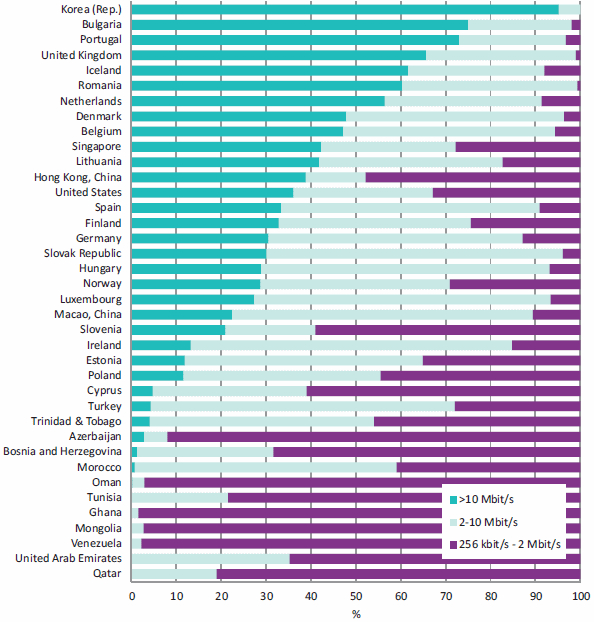
\includegraphics[bb = 0 0 594 622, scale=0.7]{broadband-speeds.jpg}%
    }
\end{figure}

% C->B: regulations' effects on BI
% talk about KC, Google Fiber, and Comcast's effect there
Romania and Estonia currently have better and cheaper Internet than the United States. The bathroom light switches in Estonia are on the outside of the bathroom and they have better Internet than the US.



% procatalepsis
% it's about cable, not the Internet (this might need to be sooner)
% "Google is competition"
Many people have argued that this deal is about cable television and has nothing to do with the Internet. This couldn't be further from the truth. Cable television is going out the door. The only real foothold that cable television currently has is sports and reality TV. Everything else can be found online. The current generation needs to die before cable television can also die, but nothing about the current merger is about cable television. It's all about Internet. According to tech pundit Paul Venezia, this merger ``is about controlling the content and delivery of Internet-based communication and entertainment.''

Paul's article on the topic will be further discussed: http://www.infoworld.com/d/data-center/the-broadband-barbarians-will-soon-control-the-gates-236847?page=0,0

% A->B (conclusion): merger's effects on BI
Historically, Comcast and Time Warner Cable have both provided terrible service and infrastructure. They've already shown that they have the infrastructure in place to provide quality bandwidth, but don't because there is no incentive. They raise prices, provide terrible customer service, and pay off the legislature to get their way. Legislation has been passed in Utah and is currently underway in Kansas to further stymie broadband infrastructure and competition. Enough is enough. Tight regulations do no allow for advancement. The United States has poorer Internet than Romania and it's because of companies like Comcast and Time Warner Cable.

\begin{workscited}
    \bibent Kessler, Andy. ``Why Super-Fast Internet Is Coming Super Slowly.'' \textit{The Wall Street Journal}. Dow Jones \& Company, 23 Feb. 2014. Web. 23 Feb. 2014.
    
    \bibent ``Question on Multi-mode Glass Fiber.'' Message to Barry M.\ Lunt. 19 Mar.\ 2014. E-mail.
    
    \bibent ``Question on Utopia.'' Message to Joseph J.\ Ekstrom. 19 Mar.\ 2014. E-mail.
    
    \bibent Romm, Tony. ``Comcast Spreads Cash Wide on Capitol Hill.'' \textit{Politico.com}. N.p., 9 Mar. 2014. Web. 12 Mar. 2014.
    
    \bibent Sottek, T. C. ``There's one thing Republicans and Democrats can agree on: taking money from Comcast.'' The Verge. N.p., 10 Mar. 2014. Web. 10 Mar. 2014.
    
    \bibent Venezia, Paul. ``The Broadband Barbarians Will Soon Control the Gates.'' \textit{InfoWorld}. N.p., 24 Feb. 2014. Web. 24 Feb. 2014.
\end{workscited}

\end{mla}
\end{document}

A: merger
v1: stymies
B: BI b/c
A': the merger
v2: creates
C: tight regulations that don't allow for advancement
